% Licence CC0 ; faites en ce que vous voulez !
\documentclass[t]{beamer}
\usepackage[latin1]{inputenc}
\usepackage[francais]{babel}
\usepackage[cyr]{aeguill}
\usepackage{setspace}
\usepackage{graphicx}
\usetheme[width=63px]{Hannover}

\date{\today}
\author{Jérémy B.}
\title{L'austérité est-elle une solution à la crise ?}

\begin{document}

\frame{\titlepage}


%Table des matières
\begin{frame}
\tableofcontents
\end{frame}
% Fin table des matières 

\section{L'austérité, pourquoi, comment ?}
\subsection{La "crise de la dette"}
\begin{frame}
	\frametitle{La "Crise de la dette"}
	La "crise de la dette" fait référence à l'explosion de la dette des \'Etats envers les banques.
	\pause
	
	\begin{center}
	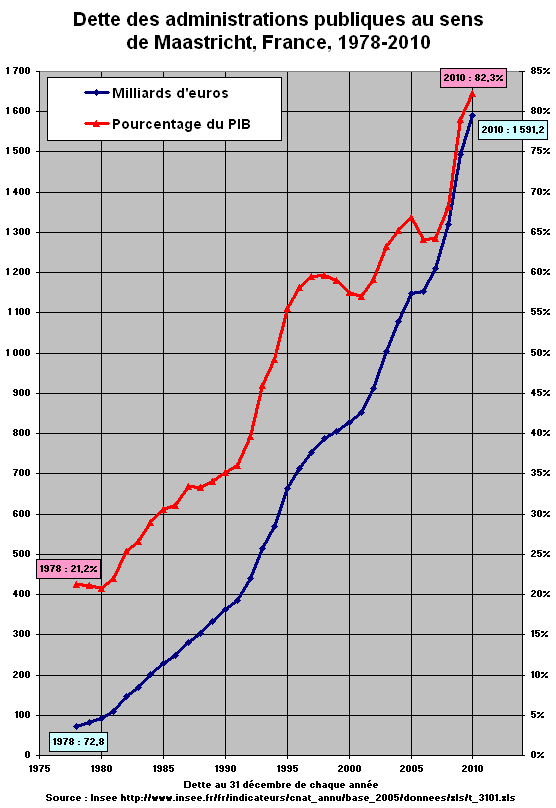
\includegraphics[width=8.5cm, height=6.8cm]{image/dette.png}
	\end{center}
	
\end{frame}

\subsection{L'austérité ou politique de rigueur}
\begin{frame}
\frametitle{L'austérité}
L'austérité est une politique qui a pour objectifs~:
\begin{itemize}
	\item de combler le déficit~;
	\pause
	\item de relancer la croissance.
	\pause
\end{itemize}

Pour cela, plusieurs moyens~:
\begin{itemize}
	\item Baisse des dépenses~;
	\pause
	\item Augmentation des taxes~;
	\pause
	\item Augmenter la "compétitivité économique".
\end{itemize}
\end{frame}

\section{L'austérité, créatrice d'inégalités}
\begin{frame}
	\frametitle{L'austérité, créatrice d'inégalités}
	L'austérité a la particularité de creuser les inégalités.
	
	\begin{center}
	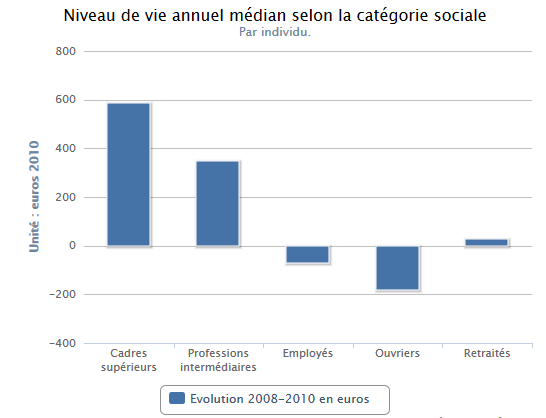
\includegraphics[width=8.5cm, height=6.8cm]{image/niveau_de_vie.png}
	\end{center}
\end{frame}

\section{L'austérité améliore-t-elle les choses ?}
\subsection{Taux de chomage en France}
\begin{frame}
	\frametitle{Taux de chomage en France}
	Depuis le début de la crise et des politiques d'austérité, le taux de chomage en France, augmente.
	
	\begin{center}
	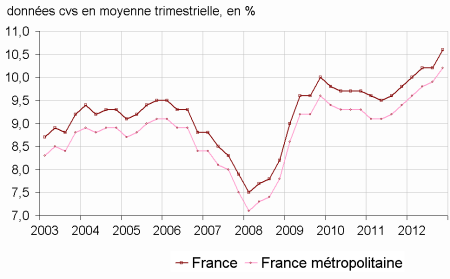
\includegraphics[width=8.5cm, height=6.8cm]{image/chomage.png}
	\end{center}
\end{frame}

\subsection{Taux de chomage en Grèce}
\begin{frame}
\frametitle{Taux de chomage en Grèce}
Grèce~: exemple parfait de l'application d'une forte politique d'austérité. \\
\pause
Le taux de chomage a explosé~:
\begin{center}
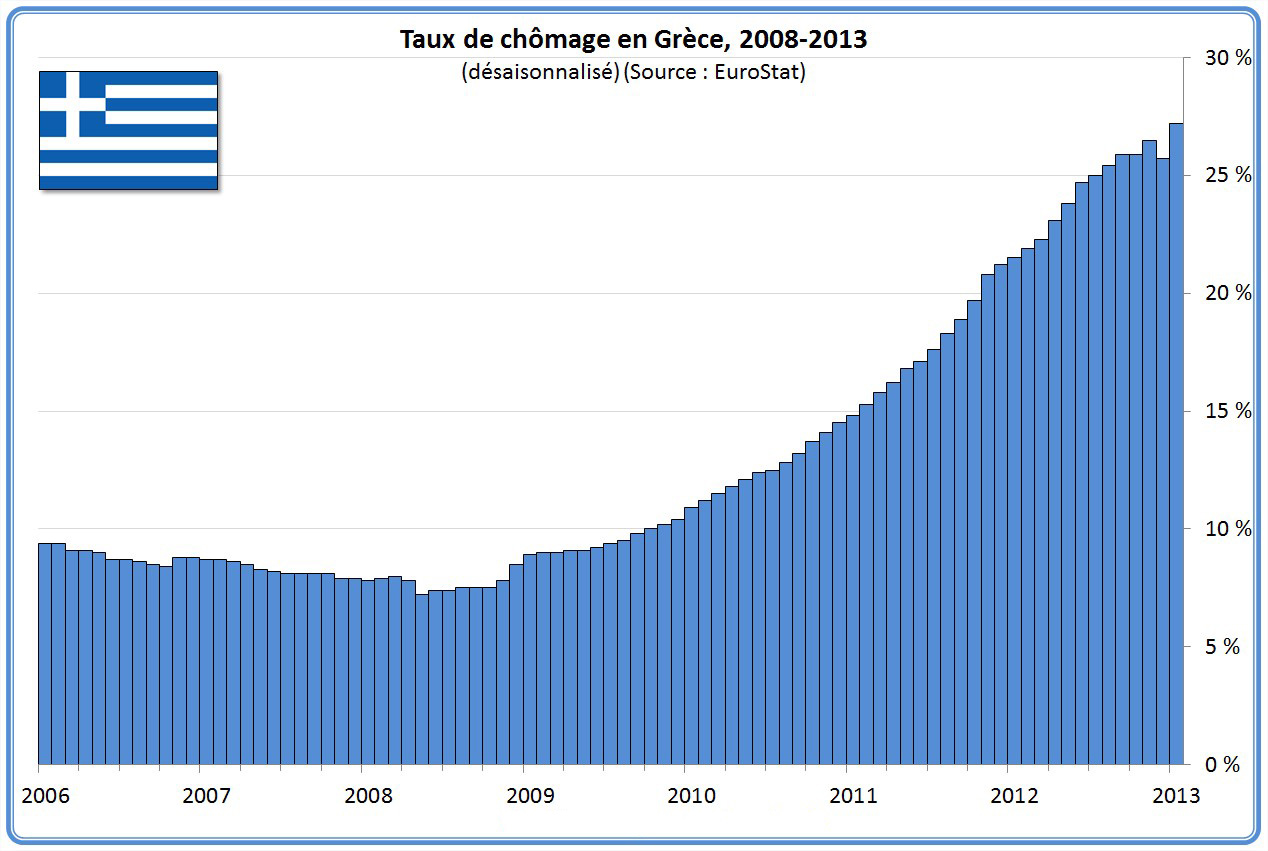
\includegraphics[width=8.5cm, height=6.8cm]{image/chomage_grece.jpg}
\end{center}
\end{frame}

\section{Conclusion}
\begin{frame}
	\frametitle{Conclusion}
	Voilà donc ce que l'on peut dire des politiques d'austérité~:
	\bigskip
	
	Baisse des dépenses -> moins d'aide -> moins de pouvoir d'achat -> moins de consommation -> moins de croissance. \\
	\pause
	Les politiques d'austérités ont donc deux objectifs contradictoire.
	\pause
	\bigskip
	
	«Il paraît que la crise rend les riches plus riches et les pauvres plus pauvres.» Coluche.

\end{frame}
\end{document}